\chapter{Introduction}

\section{Background and the nEDM Experiment}
The following description of the experiment was largely taken from \cite{EDMReport2, EDMReport, Schneider12}:\\
An electric dipole moment of a quantum system would violate time-reversal symmetry breaking effects at low energies. Assuming the conservation of CPT, violation of T also implies CP violation. Currently, such effects have only been observed in the decays particle like the K meson. However, this is by far too small to explain the observed Baryon asymmetry in the universe (BAU). As pointed out by Sakharov already in 1967, the explanation of this problem requires new sources of CP violation, baryon number non-conservation and processes out of thermal equilibrium. In addition, there is the unexplained question why the strong interaction does not violate CP, as it would naturally be expected by the CP violating product of the gluon operator and its dual within the QCD Lagrangian, weighted by a strongly restricted parameter theta. \\

Basically all popular models for physics beyond the SM, in particular Supersymmetry, naturally suggest EDMs close to the current experimental upper limits. The goal is to lower the experimental bound by  $> 100$ within the next four years, increasing the sensitivity to $ 5*10^{-28} $ ecm (3$\sigma$). \\

\begin{figure}[h!]
	\centering
	{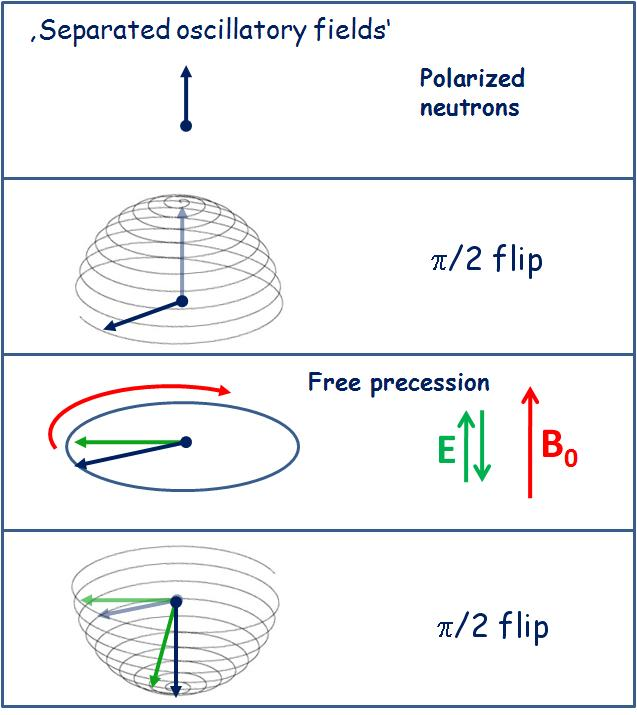
\includegraphics[width=0.4\textwidth]{images/ramsey.png}}
	\caption{Separated oscillatory fields from \cite{EDMReport}}
\end{figure}

As a measurement method the the commonly known method of separated oscillatory fields by Ramsey will be used. This is an interferometric nuclear magnetic resonance method applied to polarized and trapped ultra-cold neutrons. Spin polarized UCN precess in a highly homogeneous and constant magnetic field of 1$\mu T$. In an electric field applied along the magnetic field, a non-zero EDM would cause an additional level splitting, thus changing the Larmor frequency.\\


Ramsey's method of separated oscillatory fields: starting with an ensemble of polarized ultra-cold neutrons, the polarization is flipped into a precession plane normal to the constant field $B_{0}$. During a long period of free precession, an additional electric field E is applied parallel or anti-parallel to $B_{0}$, causing a small phase in the angle after precession. As the spin is flipped back along $B_{0}$, the deviation is analyzed. 

\section{Objectives}
The main target is to develop a prototypical implementation of a full functional data acquisition system. It should be possible to provide methods to insert data measured from devices. Those methods should be implemented in C/C++ and published through a library that supports Windows and Unix systems. Additionally a LabVIEW VI should be created that uses the functions to provide a template for upcoming implementations.\\
Furthermore, a user interface is required to visualize the stored data and to send commands to the measuring devices. Those commands or notifications should be received using event notification, especially active listening should be avoided. As a consequence to the data store that is going to be used, namely CouchDB, the user interface should be developed as a CouchApp. 